\documentclass[11pt,t, usenames, dvipsnames]{beamer}
% Theme options: kul/kulak/lrd and normal/sedes
\usetheme{kuleuven2}

%%% SETTINGS
% Use serifs font for math environments
\usefonttheme[onlymath]{serif}
% Footline on all slides
\setbeamertemplate{footline}[body]

%%% ADDED PACKAGES:
\usepackage[utf8]{inputenc}
\usepackage[english]{babel}
\usepackage{amsfonts}
\usepackage{amssymb}
\usepackage{xcolor}
\usepackage{marvosym}
\usepackage{hyperref}
\usepackage[style=authoryear]{biblatex}
% \usepackage{enumitem}

\addbibresource{bibliography.bib}
\AtEveryCite{\color{kul-blue}}
\hypersetup{colorlinks=false}


%%% TITLE PAGE INFO:
\title[Heuristic Graph Optimization using Tree Decompositions]
{\LARGE Developing Heuristic Algorithms for Graph Optimization Problems using Tree Decompositions}
\author{Louis Carpentier \newline Promotor: Jan Goedgebeur \newline Mentor: Jorik Jooken}
\institute{KU Leuven}
\date{December, 2021}

%%% TIKZ STYLE:
\tikzstyle{vertex}=[draw=black, shape=circle, thick, minimum width=0.8cm]
\tikzstyle{bag}=[draw=black, shape=ellipse, thick]
\tikzstyle{vertex_red}=[vertex, fill=Red!85]
\tikzstyle{vertex_green}=[vertex, fill=Green!85]
\tikzstyle{vertex_yellow}=[vertex, fill=YellowOrange!85]
\tikzstyle{edge}=[thick]

\tikzstyle{arrow}=[draw=kul-blue, fill=kul-blue, single arrow, minimum width=4mm, minimum height=7mm, single arrow head extend=2mm]
\newcommand{\arrowup}{%
    \tikz [baseline=-0.5ex]{\node [arrow,rotate=90] {};}
}
\newcommand{\arrowright}{%
    \tikz [baseline=-0.5ex]{\node [arrow] {};}
}
\newcommand{\arrowdown}{%
    \tikz [baseline=-1ex]{\node [arrow,rotate=-90] {};}
}

%%% EXTRA COMMANDS
\newcommand{\NP}{\mathcal{NP}}
\newcommand{\W}[1]{\mathcal{W}[#1]}
\newcommand{\T}{\mathcal{T}}
\newcommand{\bigO}{\mathcal{O}}
\newcommand{\fancyP}{\mathcal{P}}
\newcommand{\fancyH}{\mathcal{H}}

%%% OVERVIEW AT BEGINNING SECTION:
\AtBeginSection[]
{
	\begin{frame}{Overview}
	    \hfill{\large\parbox{.961\textwidth}{\tableofcontents[currentsection, hideothersubsections]}}
	\end{frame}
}


\begin{document}
% Recalculate head and foot dimension
\csname beamer@calculateheadfoot\endcsname 


% Title page
\begin{frame}[plain,noframenumbering]
	\titlepage
\end{frame}
	
% Table of Contents
\begin{frame}{Overview}
	\hfill{\large\parbox{.961\textwidth}{\tableofcontents[hideothersubsections]}}
\end{frame}



\section{Introduction}

\begin{frame}{Graph}
    \begin{columns}[c]
    \begin{column}{0.6\textwidth}
        \begin{itemize}
            \item<1-> A graph $G=(V,E)$
            \begin{itemize}
                \item vertices $V(G)$: 1, 2, 3, ...
                \item edges $E(G)$: $\{1,2\}$, $\{3,5\}$, $\{7,8\}$, ...
            \end{itemize}
            \item<2-> For all $v \in V(G)$, $deg(v)$ is the degree of vertex $v$
            \begin{itemize}
                \item $deg(3) = 4$, $deg(8) = 2$
            \end{itemize}
            \item<3-> For all $v \in V(G)$, $N(v)$ is the set of vertices $u$ such that $uv \in E(G)$
            \begin{itemize}
                \item $N(3) = \{1,2,4,5\}$, $N(8) = \{4,7\}$
            \end{itemize} 
        \end{itemize}
    \end{column}
    \begin{column}{0.4\textwidth} 
        \centering
        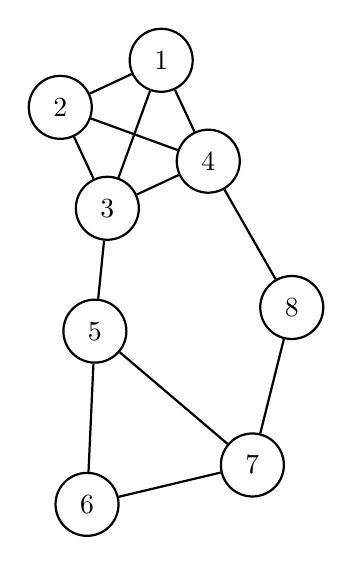
\begin{tikzpicture}
            \node[vertex] (1) at ({cos(70)},{sin(70)}) {1};
            \node[vertex] (2) at ({cos(160)},{sin(160)}) {2};
            \node[vertex] (3) at ({cos(250)},{sin(250)}) {3};
            \node[vertex] (4) at ({cos(340)},{sin(340)}) {4};
            \node[vertex] (5) at (-0.5,-2.5) {5};
            \node[vertex] (6) at (-0.6,-4.7) {6};
            \node[vertex] (7) at (1.5,-4.2) {7};
            \node[vertex] (8) at (2,-2.2) {8};
            \draw[edge] (1) -- (2);
            \draw[edge] (2) -- (3);
            \draw[edge] (3) -- (4);
            \draw[edge] (4) -- (1);
            \draw[edge] (1) -- (3);
            \draw[edge] (2) -- (4);
            \draw[edge] (3) -- (5);
            \draw[edge] (5) -- (6);
            \draw[edge] (5) -- (7);
            \draw[edge] (6) -- (7);
            \draw[edge] (8) -- (7);
            \draw[edge] (8) -- (4);
	    \end{tikzpicture}
    \end{column}
    \end{columns}
\end{frame}

\begin{frame}{Tree Decomposition}
    \begin{definition}[Tree decomposition \cite{cygan2015parameterized}]
        A \textit{tree decomposition} of graph $G$ is a pair $\T=(T, \{X_t\}_{t \in V(T)})$ where $T$ is a tree whose every node $t$ is assigned a vertex subset $X_t \subseteq V(G)$, called a bag, such that the following three conditions hold:
        \begin{enumerate}
            \item $\bigcup_{t \in V(T)} X_t = V(G)$: every vertex $v \in V(G)$ is contained in some bag $X_t$ for $t \in V(T)$.
            \item For every $\{u,v\} \in E(G)$, there exists a node $t$ of $V(T)$ such that bag $X_t$ contains both $u$ and $v$.
            \item For every $v \in V(G)$, the set $T_v = \{t \in V(T) : v \in X_t\}$ induces a connected subtree of $T$.
        \end{enumerate}
    \end{definition}
\end{frame}

\begin{frame}{}
    \vspace{0.2cm}
    \begin{example}[Property 
            \only<1>{1: $\bigcup_{t \in V(T)} X_t = V(G)$: every vertex $v \in V(G)$ is contained in some bag $X_t$ for $t \in V(T)$}%
            \only<2>{2: For every $\{u,v\} \in E(G)$, there exists a node $t$ of $V(T)$ such that bag $X_t$ contains both $u$ and $v$}%
            \only<3>{3: For every $v \in V(G)$, the set $T_v = \{t \in V(T) : v \in X_t\}$ induces a connected subtree of $T$}]
        \centering
        \begin{tikzpicture}
            \node[vertex] (1) at ({cos(70)},{sin(70)}) {1};
            \node[vertex] (2) at ({cos(160)},{sin(160)}) {2};
            \node[vertex] (3) at ({cos(250)},{sin(250)}) {3};
            \only<-2>{\node[vertex] (4) at ({cos(340)},{sin(340)}) {4};}
            \node[vertex] (5) at (-0.5,-2.5) {5};
            \node[vertex] (6) at (-0.6,-4.7) {6};
            \only<-1,3->{\node[vertex] (7) at (1.5,-4.2) {7};}
            \only<-1,3->{\node[vertex] (8) at (2,-2.2) {8};}
            \only<2>{
                \node[vertex, red] (7) at (1.5,-4.2) {7};
                \node[vertex, red] (8) at (2,-2.2) {8};
                \draw[edge, red] (8) -- (7);
            }
            \only<3>{\node[vertex, red] (4) at ({cos(340)},{sin(340)}) {4};}
            \draw[edge] (1) -- (2);
            \draw[edge] (2) -- (3);
            \draw[edge] (3) -- (4);
            \draw[edge] (4) -- (1);
            \draw[edge] (1) -- (3);
            \draw[edge] (2) -- (4);
            \draw[edge] (3) -- (5);
            \draw[edge] (5) -- (6);
            \draw[edge] (5) -- (7);
            \draw[edge] (6) -- (7);
            \draw[edge] (8) -- (4);
            \only<-1,3->{\draw[edge] (8) -- (7);}
	    \end{tikzpicture}
	    \hfil
	    \begin{tikzpicture}
	        \node[bag] (1) at (0,0) {5, 6, 7};
	        \only<-2>{\node[bag] (2) at (0,-1.5) {4, 5, 7};}
	        \only<-1>{\node[bag] (3) at (-1.5,-3) {4, 7, 8};}
	        \only<-2>{\node[bag] (4) at (1.5,-3) {3, 4, 5};}
	        \only<-2>{\node[bag] (5) at (1.5,-4.5) {1, 2, 3, 4};}
	        \only<2>{
                \node[bag, red] (3) at (-1.5,-3) {4, 7, 8};
            }
            \only<3>{
	            \node[bag, red] (2) at (0,-1.5) {4, 5, 7};
                \node[bag, red] (3) at (-1.5,-3) {4, 7, 8};
                \node[bag, red] (4) at (1.5,-3) {3, 4, 5};
                \node[bag, red] (5) at (1.5,-4.5) {1, 2, 3, 4};
                \draw[edge, red] (4) -- (5);
                \draw[edge, red] (2) -- (4);
                \draw[edge, red] (2) -- (3);
            }
	        \draw[edge] (1) -- (2);
	        \only<-2>{\draw[edge] (2) -- (3);}
	        \only<-2>{\draw[edge] (2) -- (4);}
	        \only<-2>{\draw[edge] (4) -- (5);}
	        \node at (0,-5.5) {};
	    \end{tikzpicture}
    \end{example}
\end{frame}

\begin{frame}{Treewidth}
    \begin{definition}[Width of a tree decomposition]
        The \textit{width of a tree decomposition} $\T=(T, \{X_t\}_{t \in V(T)})$ equals $max_{t \in V(T)} |X_t| - 1$.
    \end{definition}
    
    \begin{definition}[Treewidth of a graph]
        The \textit{treewidth} of a graph $G$ -- denoted by $t=tw(G)$ -- is the minimum possible width of a tree decomposition of $G$.
    \end{definition}
    
    % \begin{theorem}[\cite{cygan2015parameterized}]
    %     If a graph $G$ admits a tree decomposition of width at most $t$, then it also admits a nice tree decomposition of width at most $t$. 
    % \end{theorem}
\end{frame}

\begin{frame}{The Treewidth Problem}
    \begin{theorem}[\cite{arnborg1987complexity}]
        Given a graph $G$ and integer $t$, deciding if $G$ has a treewidth of at most $t$ is $\NP$-complete. 
    \end{theorem}
    
    \begin{itemize}
        \item<2-> Many algorithms exist for computing a tree decomposition exist 
        \begin{itemize}
            \item Exponential time exact algorithms
            \item Polynomial time approximation algorithms
            \item Heuristics with local search 
            \item See \cite{bodlaender2005discovering} for an extensive overview
        \end{itemize}
        \item<3-> PACE 2017: \cite{dell2018pace}
        \begin{itemize}
            \item Construct an algorithm to compute tree decompositions
            \item See for example \cite{tamaki2019positive, strasser2017computing, bannach2019practical}
        \end{itemize}
    \end{itemize}
\end{frame}

\begin{frame}{Nice Tree Decomposition} 
    \begin{definition}[Nice Tree Decomposition]
        A rooted tree decomposition $\T=(T, \{X_t\}_{t \in V(T)})$ of graph $G$ is \textit{nice} if the following conditions hold:
        \begin{itemize}
            \item $X_r = \emptyset$ and $X_l = \emptyset$ for every leaf $l$ of $V(T)$.
            \item Every non-leaf node of $T$ is one of the following types:
            \begin{enumerate}
                \item Introduce node: a node $t$ with exactly 1 child $t'$ such that $X_t = X_{t'} \cap \{v\}$ for some vertex $v \not\in X_{t'}$.
                \item Forget node: a node $t$ with exactly 1 child $t'$ such that $X_t = X_{t'} \setminus \{v\}$ for some vertex $v \in X_{t'}$.
                \item Join node: a node $t$ with exactly two children $t_1, t_2$ such that $X_t = X_{t_1} = X_{t_2}$
            \end{enumerate}
        \end{itemize}
    \end{definition}
\end{frame}

\begin{frame}{}
    \vspace{0.2cm}
    \begin{example}[\only<1>{Root and leaves}\only<2>{Introduce node}\only<3>{Forget node}\only<4>{Join node}]
        \centering
        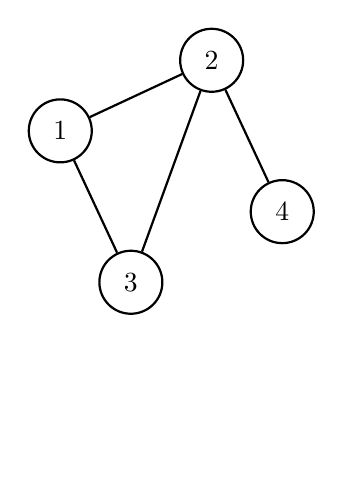
\begin{tikzpicture}
            \node[vertex] (1) at ({1.5*cos(160)},{1.5*sin(160)}) {1};
            \node[vertex] (2) at ({1.5*cos(70)},{1.5*sin(70)}) {2};
            \node[vertex] (3) at ({1.5*cos(250)},{1.5*sin(250)}) {3};
            \node[vertex] (4) at ({1.5*cos(340)},{1.5*sin(340)}) {4};
            \draw[edge] (1) -- (2);
            \draw[edge] (1) -- (3);
            \draw[edge] (2) -- (3); 
            \draw[edge] (2) -- (4); 
            \node at (0,-3.5) {};
        \end{tikzpicture}
        \hfil
        \begin{tikzpicture}
            \only<2->\node[bag] (1) at (0,0) {};
            \only<-1>\node[bag, red] (1) at (0,0) {};
            \node[bag] (2) at (0,-0.8) {1};
            \only<-3>\node[bag] (3) at (0,-1.8) {1,2};
            \only<4>\node[bag, red] (3) at (0,-1.8) {1,2};
            \only<-3>\node[bag] (4) at (-2,-2.8) {1,2};
            \only<4>\node[bag, Green] (4) at (-2,-2.8) {1,2};
            \only<-1,3->\node[bag] (5) at (-2,-3.8) {1,2,3};
            \only<2>\node[bag, red] (5) at (-2,-3.8) {1,2,3};
            \only<-1,3->\node[bag] (6) at (-2,-4.8) {1,3};
            \only<2>\node[bag, Green] (6) at (-2,-4.8) {1,3};
            \node[bag] (7) at (-2,-5.8) {1};
            \only<2->\node[bag] (8) at (-2,-6.8) {};
            \only<-1>\node[bag, red] (8) at (-2,-6.8) {};
            \only<-3>\node[bag] (9) at (2,-2.8) {1,2};
            \only<4>\node[bag, Green] (9) at (2,-2.8) {1,2};
            \only<-2,4>\node[bag] (10) at (2,-3.8) {2};
            \only<3>\node[bag, red] (10) at (2,-3.8) {2};
            \only<-2,4>\node[bag] (11) at (2,-4.8) {2,4};
            \only<3>\node[bag, Green] (11) at (2,-4.8) {2,4};
            \node[bag] (12) at (2,-5.8) {4};
            \only<2->\node[bag] (13) at (2,-6.8) {};
            \only<-1>\node[bag, red] (13) at (2,-6.8) {};
            \draw[edge] (1) -- (2);
            \draw[edge] (2) -- (3);
            \only<-3>\draw[edge] (3) -- (4);
            \only<4>\draw[edge, Green] (3) -- (4);
            \draw[edge] (4) -- (5);
            \only<-1,3->\draw[edge] (5) -- (6);
            \only<2>\draw[edge, Green] (5) -- (6);
            \draw[edge] (6) -- (7);
            \draw[edge] (7) -- (8);
            \only<-3>\draw[edge] (3) -- (9);
            \only<4>\draw[edge, Green] (3) -- (9);
            \draw[edge] (9) -- (10);
            \only<-2,4>\draw[edge] (10) -- (11);
            \only<3>\draw[edge, Green] (10) -- (11);
            \draw[edge] (11) -- (12);
            \draw[edge] (12) -- (13);
	    \end{tikzpicture}
    \end{example}
\end{frame}

\begin{frame}{Dynamic Programming using Nice Tree Decompositions}
    \begin{itemize}
        \item<1-> Define cost $\tau[t, X]$ at every node of $t \in V(T)$ 
        \begin{itemize}
            \item $X$ depends on the problem
        \end{itemize}
        \item<2-> Compute $\tau[t, X]$ in a bottom-up fashion
        \begin{itemize}
            \item Bags can only relate in a few simple ways to the bags of the children in a nice tree decomposition
        \end{itemize}
        \item<3-> Final evaluation is $\tau[r,\emptyset]$ for root $r$ of $T$
        \only<4->{
            \vspace{0.3cm}
            \item<4-> Results in time complexity of $\bigO(c^{\bigO(tw(G))} \cdot n^{\bigO(1)})$
            \item<5-> What if the constraint of an exact solution is dropped in order to reduce the exponential term in $tw(G)$?
            
            \only<6-> {
                \arrowright Goal of my thesis
            }
        }
    \end{itemize}
    
    % \only<4> {
    %     \begin{theorem}[\cite{cygan2015parameterized}]
    %         Given tree decomposition $\T=(T, \{X_t\}_{t \in V(T)})$ of a graph $G$. For any edge $uv \in E(T)$, then $X_u \cap X_v$ is a separator for $G$.
    %     \end{theorem}
    % }
    
\end{frame}

% \begin{frame}{}
%     \vspace{0.2cm}
%     \begin{example}[Maximum Happy Vertices \cite{agrawal2017parameterized}]
%         Define cost $\tau[t, \fancyP, \fancyH]$
%         \begin{itemize}
%             \item $\fancyP = (P_1 \dots P_k)$ is a partition of $X_t$ into $k$ sets
%             \item $\fancyH = \{(H_i, U_i) | H_i \uplus U_i = P_i \}$ is a set of pairs which split $P_i$ into the vertices that are happy and those that are unhappy
%         \end{itemize}
        
%         \vspace{0.2cm}
%         Given tree decomposition $\T=(T, \{X_t\}_{t \in V(T)})$ of graph $G$
%         \begin{itemize}
%             \item consider all $\tau[t, \fancyP, \fancyH]$
%             \item At node $t$, there are $\bigO(k^{|X_t|})$ possible table entries
%             \item The algorithm has a running time of $\bigO(2^{\bigO(k+tw(G)log(k))}|V(G)|)$
%         \end{itemize}
        
%         \vspace{0.2cm}
%         The algorithm has a linear running time for graphs with constant treewidth $tw(G)$ on an instance with a constant number of colours $k$. 
        
%         \vspace{0.2cm}
%         \only<2->{
%             What if the constraint of an exact solution is dropped in order to reduce the exponential term in $tw(G)$?
%         }
%     \end{example}
% \end{frame}




\section{Maximum Happy Vertices}

\begin{frame}{Maximum Happy Vertices Problem (\cite{zhang2015algorithmic})}
    \begin{definition}<1->[Happy and Unhappy Vertices]
		Given a graph $G$ and a colouring $c:V(G)\rightarrow \{1 \dots k\}$. A vertex $v \in V(G)$ is said to be \textit{happy} if and only if $c(v) = c(v')$ for all vertices $v' \in N(v)$, otherwise vertex $v$ is said to be \textit{unhappy}. 
	\end{definition}
	\begin{definition}<2->[Maximum Happy Vertices Problem -- MHV]
		Given a graph $G$ and a partial colouring $c:V(G)\rightarrow \{1 \dots k\}$. Extend the partial colouring $c$ to a full colouring $c'$ such that the number of happy vertices is maximized.
	\end{definition}
	\begin{definition}<3->[$k$-MHV]
	    An instance of the MHV problem, in which the number of colours $k$ is a constant. 
	\end{definition}
\end{frame} 

\begin{frame}{}
    \vspace{0.2cm}
	\begin{example}
	    \centering
		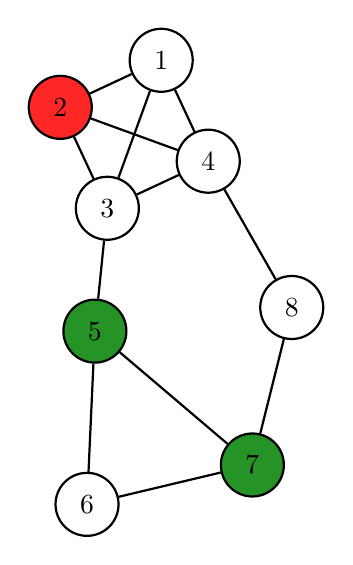
\begin{tikzpicture}
            \node[vertex] (1) at ({cos(70)},{sin(70)}) {1};
            \node[vertex_red] (2) at ({cos(160)},{sin(160)}) {2};
            \node[vertex] (3) at ({cos(250)},{sin(250)}) {3};
            \node[vertex] (4) at ({cos(340)},{sin(340)}) {4};
            \node[vertex_green] (5) at (-0.5,-2.5) {5};
            \node[vertex] (6) at (-0.6,-4.7) {6};
            \node[vertex_green] (7) at (1.5,-4.2) {7};
            \node[vertex] (8) at (2,-2.2) {8};
            \draw[edge] (1) -- (2);
            \draw[edge] (2) -- (3);
            \draw[edge] (3) -- (4);
            \draw[edge] (4) -- (1);
            \draw[edge] (1) -- (3);
            \draw[edge] (2) -- (4);
            \draw[edge] (3) -- (5);
            \draw[edge] (5) -- (6);
            \draw[edge] (5) -- (7);
            \draw[edge] (6) -- (7);
            \draw[edge] (8) -- (7);
            \draw[edge] (8) -- (4);
	    \end{tikzpicture}
	    \hspace{0.2cm}
	    \begin{tikzpicture}
	        \node at (0,2.75) {};
	        \node at (0,0) {$\longrightarrow$};
	        \node at (0,-2.75) {};
	    \end{tikzpicture}
	    \hspace{0.2cm}
	    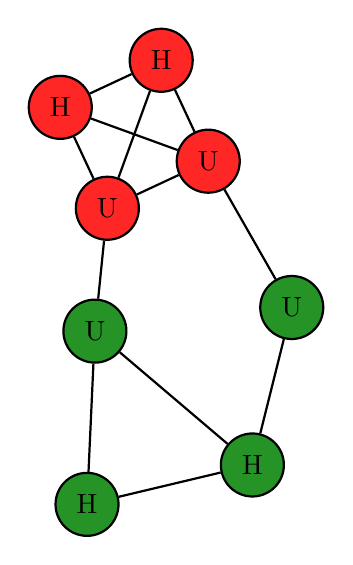
\begin{tikzpicture}
            \node[vertex_red] (1) at ({cos(70)},{sin(70)}) {H};
            \node[vertex_red] (2) at ({cos(160)},{sin(160)}) {H};
            \node[vertex_red] (3) at ({cos(250)},{sin(250)}) {U};
            \node[vertex_red] (4) at ({cos(340)},{sin(340)}) {U};
            \node[vertex_green] (5) at (-0.5,-2.5) {U};
            \node[vertex_green] (6) at (-0.6,-4.7) {H};
            \node[vertex_green] (7) at (1.5,-4.2) {H};
            \node[vertex_green] (8) at (2,-2.2) {U};
            \draw[edge] (1) -- (2);
            \draw[edge] (2) -- (3);
            \draw[edge] (3) -- (4);
            \draw[edge] (4) -- (1);
            \draw[edge] (1) -- (3);
            \draw[edge] (2) -- (4);
            \draw[edge] (3) -- (5);
            \draw[edge] (5) -- (6);
            \draw[edge] (5) -- (7);
            \draw[edge] (6) -- (7);
            \draw[edge] (8) -- (7);
            \draw[edge] (8) -- (4);
		\end{tikzpicture}
	\end{example}
\end{frame}
	
\begin{frame}{Applications of Maximum Happy Vertices}
    \begin{enumerate}
        \item<1-> Modeling social networks: \textit{homophyly}
        \begin{itemize}
            \item People tend to be similar to their friends
            \item Elements in a small community share remarkable common features
            \item The feature values are represented by a colour
            \item See \cite{easley2010networks, li2011community, li2012small} for more information
        \end{itemize}
        
        \item<2-> Clustering 
        \begin{itemize}
            \item The vertices represent data points
            \item The edges represent strong connections between the data points
            \item The colours represent the different clusters
        \end{itemize}
    \end{enumerate}
\end{frame}

\begin{frame}{Complexity of the Maximum Happy Vertices Problem}
    \only<1->{
        \begin{theorem}[\cite{zhang2015algorithmic}]
    		The $k$-MHV problem is $\NP$-complete for every constant $k \geq 3$.
    	\end{theorem}
    }

    \only<2->{
        \begin{theorem}<2->[\cite{aravind2017algorithms}]
            The $k$-MHV problem is $\NP$-complete for split graphs and bipartite graphs for every constant $k \geq 3$.
        \end{theorem} 
    }
    
    \only<2> {
        \begin{columns}
        \begin{column}{0.5\textwidth}
            \centering
            \begin{tikzpicture}
                \node[vertex] (1) at ({1.2*cos(30)}, {1.2*sin(30)}) {1};
                \node[vertex] (2) at ({1.2*cos(120)}, {1.2*sin(120)}) {2};
                \node[vertex] (3) at ({1.2*cos(210)}, {1.2*sin(210)}) {3};
                \node[vertex] (4) at ({1.2*cos(300)}, {1.2*sin(300)}) {4};
                \draw[edge] (1) -- (2);
                \draw[edge] (1) -- (3);
                \draw[edge] (1) -- (4);
                \draw[edge] (2) -- (3);
                \draw[edge] (2) -- (4);
                \draw[edge] (3) -- (4);
                \draw[dashed, kul-blue, ultra thick, rounded corners] (1.7,1.7) rectangle (-1.7,-1.7);
                
                \node[vertex] (5) at (3,1.1) {5};
                \node[vertex] (6) at (3,0) {6};
                \node[vertex] (7) at (3,-1.1) {7};
                \draw[edge] (5) -- (1);
                \draw[edge] (5) -- (2);
                \draw[edge] (6) -- (3);
                \draw[edge] (7) -- (1);
                \draw[edge] (7) -- (4);
                \draw[dashed, kul-blue, ultra thick, rounded corners] (2.2,1.7) rectangle (3.8,-1.7);
            \end{tikzpicture}
        \end{column}
        \begin{column}{0.5\textwidth}
            \centering
            \begin{tikzpicture}
                \node[vertex] (1) at (0.5, 0.7) {1};
                \node[vertex] (2) at (0.5,-0.7) {2};
                \draw[dashed, kul-blue, ultra thick, rounded corners] (-0.3,1.7) rectangle (1.3,-1.7);
                
                \node[vertex] (3) at (3,1.1) {3};
                \node[vertex] (4) at (3,0) {4};
                \node[vertex] (5) at (3,-1.1) {5};
                \draw[dashed, kul-blue, ultra thick, rounded corners] (2.2,1.7) rectangle (3.8,-1.7);
                
                \draw[edge] (1) -- (3);
                \draw[edge] (1) -- (4);
                \draw[edge] (2) -- (3);
                \draw[edge] (2) -- (5);
            \end{tikzpicture}
        \end{column}
        \end{columns}
    }
    
    \only<3->{
        \begin{theorem}<3->[\cite{agrawal2017parameterized}]
    		The MHV problem when parametrized by the number of happy vertices is $\W{1}$-hard.
    	\end{theorem}
    }
\end{frame}




\section{A Heuristic Algorithm using Nice Tree Decompositions}

\begin{frame}{Heuristic Approach}
    \begin{itemize}
        \item What causes the exponential term in the running time?
        \begin{itemize}
            \item<2-> Due to the size of the dynamic programming table
        \end{itemize}
    \end{itemize}
    
    \only<3-> {
        \vspace{0.5cm}
        \begin{columns}[c]
        \begin{column}{0.6\textwidth}
            \begin{itemize}
                \item Compute a fixed number of colour functions at each node
                \item Colour functions at node $t$ contain information about $X_{t'}$ for all descendants $t'$ of $t$
                \begin{itemize}
                    \item Descendants of $t_3$: $\{t_4\}$
                    \item Descendants of $t_2$: $\{t_3, t_4, t_5\}$
                \end{itemize}
            \end{itemize}
        \end{column}
        \begin{column}{0.4\textwidth}
            \centering
            \begin{tikzpicture}
                \node[bag] (1) at (0,0) {$t_1$};
                \node[bag] (2) at (0,-1.2) {$t_2$};
                \node[bag] (3) at (-1.2,-2.4) {$t_3$};
                \node[bag] (4) at (-1.2,-3.6) {$t_4$};
                \node[bag] (5) at (1.2,-2.4) {$t_5$};
                \draw[edge] (1) -- (2);
                \draw[edge] (2) -- (3);
                \draw[edge] (2) -- (5);
                \draw[edge] (3) -- (4);
            \end{tikzpicture}
        \end{column}
        \end{columns}
    }
\end{frame}

\begin{frame}{Leaf Nodes}
    \begin{columns}[c]
    \begin{column}{0.7\textwidth}
        \begin{itemize}
            \item Leaf nodes have empty bags
            \vspace{0.2cm}
            \newline\arrowright Pass initial colour function to parent
        \end{itemize}
    \end{column}
    \begin{column}{0.3\textwidth} 
        \centering
        \begin{tikzpicture}
            \node[bag] (1) at (0,0) {$\emptyset$};
            \node (2) at (0,1.2) {};
            \draw[edge, dashed] (1) -- (2);
	    \end{tikzpicture}
    \end{column}
    \end{columns}
    
    \only<2->{
        \vspace{1cm}
        {\usebeamerfont{frametitle}\usebeamercolor[fg]{frametitle}\fontsize{12}{13} \textbf{Forget Nodes}}
        \begin{columns}[c]
        \begin{column}{0.7\textwidth}
            \begin{itemize}
                \item Vertex $v$ is 'forgotten' from the tree decomposition
                \item Sub tree contains the same vertices 
                \vspace{0.2cm}
                \newline\arrowright Pass colour functions of child to parent
            \end{itemize}
        \end{column}
        \begin{column}{0.3\textwidth} 
            \centering
            \begin{tikzpicture}
                \node[bag] (1) at (0,0) {$X_t \setminus \{v\}$};
                \node[bag] (2) at (0,-1.2) {$X_t$};
                \node (3) at (0,1.2) {};
                \node (4) at (0,-2.4) {};
                \draw[edge] (1) -- (2);
                \draw[edge, dashed] (1) -- (3);
                \draw[edge, dashed] (2) -- (4);
    	    \end{tikzpicture}
        \end{column}
        \end{columns}
    }
\end{frame}

\begin{frame}{Introduce Nodes}
    \begin{columns}[c]
    \begin{column}{0.7\textwidth}
        \begin{itemize}
            \item New information introduced: vertex $v$
            \begin{itemize}
                \item $v$ must receive a colour
            \end{itemize}
        \end{itemize}
        \vspace{0.3cm}
        \onslide<2->{
            Two approaches:
            \begin{enumerate}
                \item<3-> For each colour function of child, give $v$ the colour that results in the most happy vertices
                \item<4-> For each colour function of child, give $v$ all the possible colours and select the best colour functions
            \end{enumerate}
        }
    \end{column}
    \begin{column}{0.3\textwidth} 
        \centering
        \begin{tikzpicture}
            \node[bag] (1) at (0,0) {$X_t \cup \{v\}$};
            \node[bag] (2) at (0,-1.2) {$X_t$};
            \node (3) at (0,1.2) {};
            \node (4) at (0,-2.4) {};
            \draw[edge] (1) -- (2);
            \draw[edge, dashed] (1) -- (3);
            \draw[edge, dashed] (2) -- (4);
	    \end{tikzpicture}
    \end{column}
    \end{columns}
\end{frame}

\begin{frame}{Join Nodes}
    \begin{columns}[c]
    \begin{column}{0.7\textwidth}
        \begin{itemize}
            \item The left and right children pass different colour functions to the join node
            \item Merge all colour functions $c_l$ of the left child with all colour functions $c_r$ of the right child
            \item Iterate over all vertices $v \in X_t$ and assign it a colour
            \vspace{0.2cm}
        \end{itemize}
    \end{column}
    \begin{column}{0.3\textwidth} 
        \centering
        \begin{tikzpicture}
            \node[bag] (1) at (0,0) {$X_t$};
            \node[bag] (2) at (1.2,-1.2) {$X_t$};
            \node[bag] (3) at (-1.2,-1.2) {$X_t$};
            \node (4) at (0,1.2) {};
            \node (5) at (1.2,-2.4) {};
            \node (6) at (-1.2,-2.4) {};
            \draw[edge] (1) -- (2);
            \draw[edge] (1) -- (3);
            \draw[edge, dashed] (1) -- (4);
            \draw[edge, dashed] (2) -- (5);
            \draw[edge, dashed] (3) -- (6);
	    \end{tikzpicture}
    \end{column}
    \end{columns}
    \only<2->{
        Order to iterate over the vertices in $X_t$?
        \begin{enumerate}
            \item Static: random, greatest degree first, smallest degree first
            \item Dynamic: vertex connected to most/fewest already coloured vertices, vertex with fewest differently coloured neighbours
        \end{enumerate}
    }
\end{frame}

\begin{frame}{Evaluation method}
    How to decide what the best colour function is?
    \begin{enumerate}
        \item Count the number of happy vertices
        \item<4-> Count the number of happy and potentially happy vertices
    \end{enumerate}
    
    \only<2->{
        \vspace{0.6cm}
        \begin{columns}
        \begin{column}{0.5\textwidth}
            \centering
            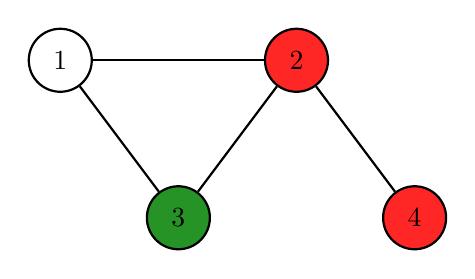
\begin{tikzpicture}
                \node[vertex] (1) at (0,0) {1};
                \node[vertex_red] (2) at (3,0) {2};
                \node[vertex_green] (3) at (1.5,-2) {3};
                \node[vertex_red] (4) at (4.5,-2) {4};
                \draw[edge] (1) -- (2);
                \draw[edge] (1) -- (3);
                \draw[edge] (2) -- (3);
                \draw[edge] (2) -- (4);
            \end{tikzpicture}
            
            \vspace{0.2cm}
            \only<3->{vertex 4 is happy, but the other vertices can never be happy} 
        \end{column}
        \begin{column}{0.5\textwidth}
            \centering
            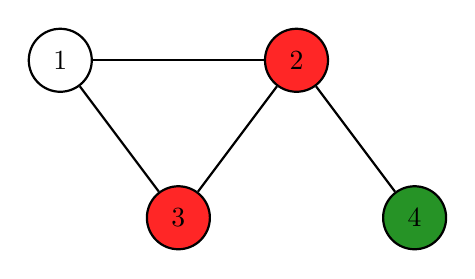
\begin{tikzpicture}
                \node[vertex] (1) at (0,0) {1};
                \node[vertex_red] (2) at (3,0) {2};
                \node[vertex_red] (3) at (1.5,-2) {3};
                \node[vertex_green] (4) at (4.5,-2) {4};
                \draw[edge] (1) -- (2);
                \draw[edge] (1) -- (3);
                \draw[edge] (2) -- (3);
                \draw[edge] (2) -- (4);
            \end{tikzpicture}
            
            \vspace{0.2cm}
            \only<3->{No vertex is happy, but both vertex 1 and 3 are happy if vertex 1 is coloured red}
        \end{column}
        \end{columns}
    }
\end{frame}


\section{Future Work}

\begin{frame}{Future Work}
    \only<1->{
        Algorithm improvement:
        \begin{itemize}
            \item Implement more techniques to handle the different types of nodes
            \item Apply kernelization on the input graph \cite{gao2018kernelization}
        \end{itemize}
    }
    
    \only<2->{
        \vspace{0.3cm}
        Experimental analysis:
        \begin{itemize}
            \item Compare algorithm performance against other, existing heuristic algorithms
            \item Compare the influence on both solution quality and running time for different tree decompositions
            \item Compare the retrieved colouring functions of the heuristic approach and exact algorithm at each node $t$ of the tree decomposition
            \item Apply \textit{framework} on other problems
        \end{itemize}
    }
\end{frame}



\begin{frame}[c,plain,noframenumbering]
    \begin{tikzpicture}[remember picture,overlay]
    \fill[fill=kul-blue]
        (current page.south east)  rectangle  ([shift={(0,-0.1\paperheight)}]current page.north west);
    \end{tikzpicture}
    
    \centering
    \vspace{1.5cm}
    \textcolor{white}{\huge Thank you for your attention!}
\end{frame}

\begin{frame}[allowframebreaks]{Bibliography}
    \nocite{*}
    \printbibliography
\end{frame}


\end{document}